% Définition du nom du chapitre
\chapter{Chapitre 5: Monitoring } \label{chapitre5-capferrat}

\pagestyle{main}

%%%%%%%%%%%%%%%%%%%%%%%%%%%%%
%%% Figure cover chapitre %%%
%%%%%%%%%%%%%%%%%%%%%%%%%%%%%
\begin{tikzpicture}
  \def\ig{%
   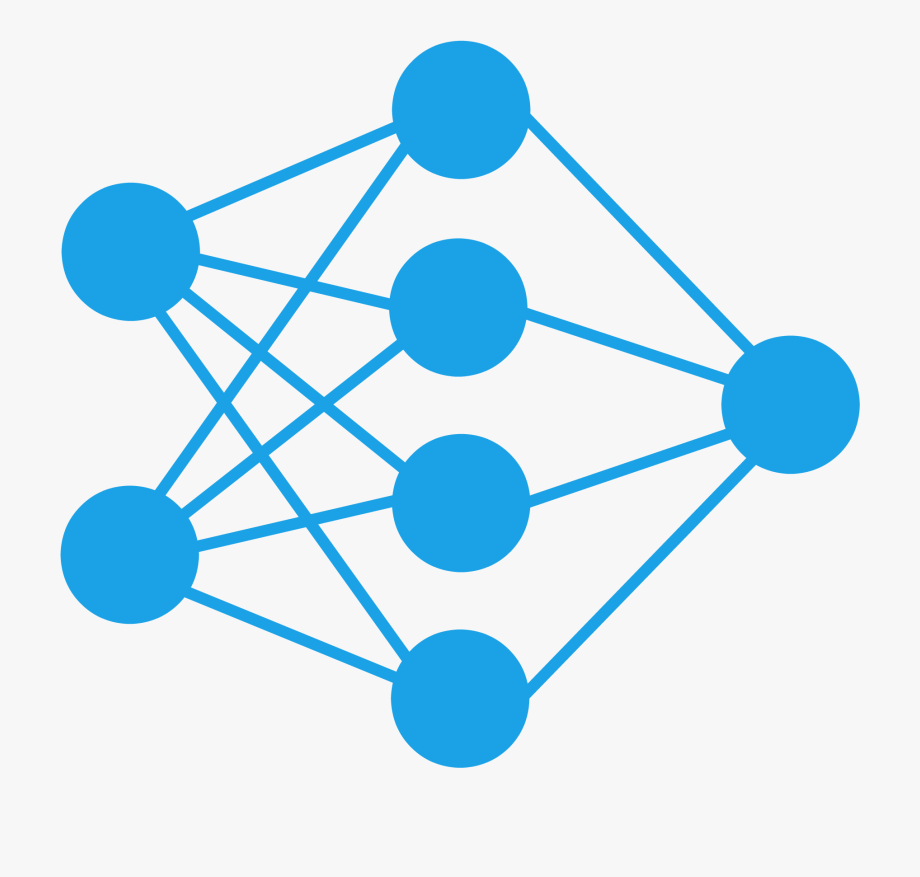
\includegraphics[width=\linewidth,keepaspectratio]{./7_chapitre5/cover}}
 \node [inner sep=0pt](mypicture) at (0,0) {\phantom{\ig}};
 \clip[rounded corners=5mm] ($(mypicture.south west)+(\bord,\bord)$) rectangle ($(mypicture.north east)-(\bord,\bord)$);
 \node[inner sep=0pt](mypicture) at (0,0) {\ig};
\end{tikzpicture}

% Bullet points du début de chapitre
\begin{center}
\begin{colbox}{resume}
  \vspace{-2pt}
{\color{textresume}\small
\begin{itemize}[leftmargin=0in]\itemsep3pt
\item les garrigues sont des milieux naturels méditerranéens ouverts, caractérisés par une végétation très hétérogène~;
\item cette hétérogénéité se caractérise par l'assemblage en mosaïque de quatre strates verticales à une échelle très fine~: le sol nu, l'herbe, les ligneux bas et les ligneux hauts~;
\item l'hétérogénéité de cette mosaïque varie de manière continue dans le paysage~;
\item cette hétérogénéité est associée à une très forte biodiversité floristique et faunistique~;
\item cette hétérogénéité est la résultante~:
\begin{itemize}
  \item d'une importante variabilité climatique et topographique~;
  \item d'activités humaines qui ont façonné les milieux de garrigues~;
\end{itemize}
\end{itemize}
}
\vspace{-2pt}
%\end{fullminipage}
\end{colbox}
\end{center}

\clearpage

\noindent\textbf{Fine scale monitoring of living Posidonia oceanica}

% Auteurs
\noindent Guilhem Marre, Florian Holon, Sandra Luque, Pierre Boissery et Julie Deter

% NB sans indentation
\noindent\textit{En cours de révision dans...}

\noindent\textbf{Abstract}


\noindent\textbf{Keywords}


\section{Introduction}\label{chapitre5_1}

\section{Materials and methods}\label{chapitre5_2}

\section{Results}\label{chapitre5_3}

\section{Discussion}\label{chapitre5_4}

\section{Conclusion}\label{chapitre5_5}
